\documentclass[11pt, a4paper]{article}

\usepackage{amsmath}
\usepackage{amsfonts}
\usepackage{physics}
\usepackage{geometry}
\usepackage{graphicx}

\geometry{top=0cm, margin=1.5cm}
\begin{document}
	\author{Aayush Arya}
	\title{Hall effect measurements for a Ge sample}
	\maketitle
	
	\hline
	\begin{center}
		PHY369 WTP Report\\
		Registration Number: 11912610 \quad Section: G2903
	\end{center}
	\hline
	
	\section*{Results}
	The values measured are as follows
	
	\begin{table}[h]
		\centering
		\begin{tabular}{|c|c|c|}
			\hline
			Hall current & $V_H$ ($B=0.4447$) & $V_H$ ($B=0.7441 $)\\
			\hline
			2.0 & 34.507 & 57.511\\
			2.5 & 43.133 & 71.889\\
			3.0 & 51.760 & 86.267 \\
			3.5 & 60.387 & 108.645\\
			4.0 & 68.014 & 115.625\\
			4.5 & 77.640 & 129.4 \\
			5.0 & 86.267 & 143.778\\
			\hline
		\end{tabular}
		\caption{Measurements for Ge, thickness=0.5mm}
	\end{table}

The data has been plotted in the figure below.
	
	\begin{figure}[!h]
		\centering
		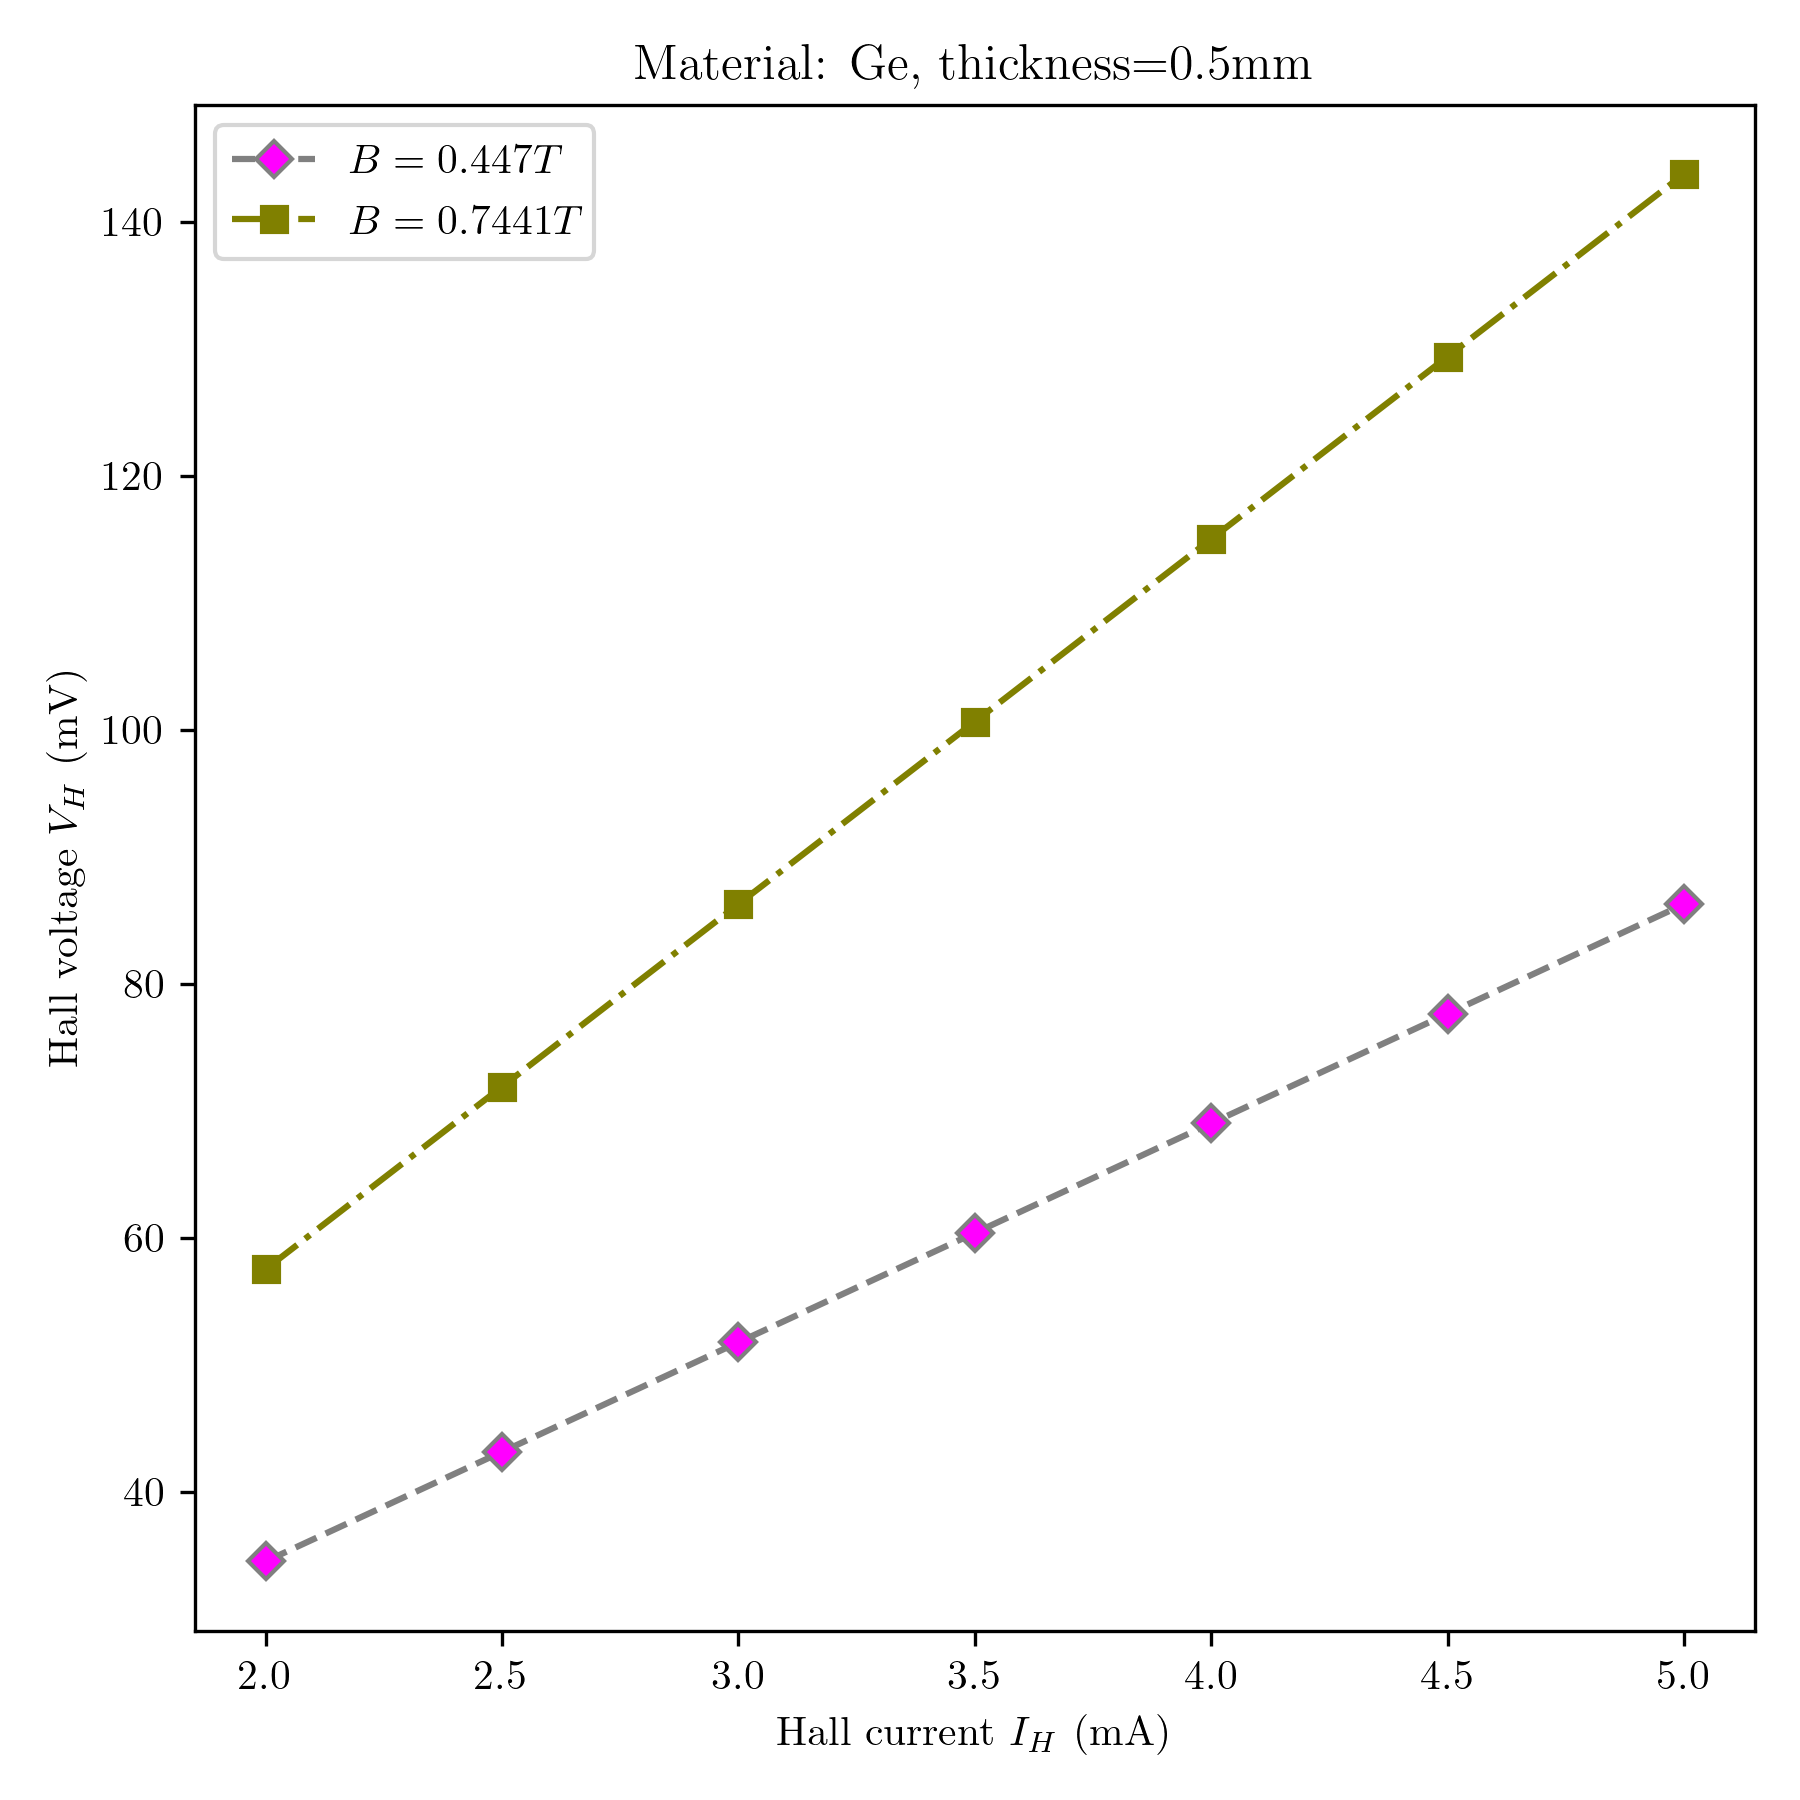
\includegraphics[width=0.6\textwidth]{../hall_effect}
		\caption{Plot of hall voltage vs current}
	\end{figure}
	
	Since the hall voltage and hall current are related by $$ V_H = \frac{R_H I B}{t} $$ where $$ R_H = \pm \frac{1}{ne}$$
	The values for $R_H$ and $n$ could be estimated from the slope of the data.\\
	
	The calculated values of $R_H$ and carrier concentration $n$ are $0.01939$ and $3.221\times 10^{20}$ respectively. The carriers are holes as the estimated value of $R_H$ is positive, which implies p-type material.\\
	
	The plots were made in Python (script available on request).
	
\end{document}